\documentclass[12pt]{article}
\usepackage[utf8]{inputenc}
\usepackage[a4paper,margin=1in]{geometry}
\usepackage{amsmath} 
\usepackage{graphicx}
\usepackage{float}
% \usepackage{tabularx} 
% \usepackage{caption}
% \usepackage{subcaption}
% \usepackage{array}
\usepackage[driverfallback=hypertex]{hyperref}
\hypersetup{colorlinks=true,urlcolor=blue,linkcolor=black}
\usepackage[numbered]{matlab-prettifier}
\usepackage{tabularx}
\newcommand\setrow[1]{\gdef\rowmac{#1}#1\ignorespaces}
\newcommand\clearrow{\global\let\rowmac\relax}
\usepackage{biblatex}

\date{}

\begin{document}

\pagenumbering{gobble}
\vspace{2cm}
\begin{center}
\centering
\begin{Huge}
    Indian Institute Of Technology Madras
\end{Huge}
 
    \begin{figure}[htp]
        \centering
        \includegraphics[width=8cm]{IITM logo.png}
    \end{figure}
\vspace{2cm}
\begin{Large}
     \textbf{\\HS4011: Econometrics\\}
        Term Project\\
\end{Large}
\vspace{1cm}
\begin{Large}
    Carbon Pricing and related factors affecting Greenhouse emissions
\end{Large}
    
\end{center}
\vspace{2cm}
\begin{large}
    \begin{table}[H]
    \centering
    \begin{tabular}{ll}
    Medhaa Priya & HS20H026\\
    D.Joseph & HS19H018\\
    Ankem Hema Srikar & AE20B012\\
    Mannem S V Sayi Teja Reddy & ME20B108 \\
    Samrudha Lakshmi V & ME20B155\\
    \end{tabular}
\end{table}
\end{large}

\newpage
\pagenumbering{arabic}

\tableofcontents 
\listoffigures
\newpage

\section{Abstract}
\paragraph{}
This paper aims to develop a multiple linear regression model to assess the impact of carbon pricing mechanism on carbon emissions. The categories of mechanism include both EU ETS (Emission Trading System) and carbon taxes adopted by different countries at the domestic level. For a more holistic analysis, the model also includes other factors that act as proxy for aspects like economic growth, energy consumption and trade openness. It further aims to test the accuracy with the existing literature and frameworks, to derive further insights and recommendations.


\section{Introduction}
\paragraph{}
In the current epoch characterized by the intensification of apprehensions about climate change, implementing efficacious measures aimed at curtailing carbon emissions has emerged as a worldwide need. Carbon pricing mechanisms are widely recognized as practical tools for promoting environmental sustainability. These mechanisms are considered fundamental techniques for incorporating the actual costs associated with carbon emissions. The concept of carbon pricing, which includes both cap-and-trade systems and carbon taxes, aims to incorporate the external cost associated with carbon emissions into economic decision-making processes. The European Union Emissions Trading System (EU ETS) operates as a cap-and-trade mechanism whereby it establishes a predetermined limit on greenhouse gas emissions and enables participating organizations to trade emission permits.
\\[\baselineskip]
Conversely, carbon taxes provide a tangible cost for carbon emissions, creating a monetary motivation for enterprises to mitigate their carbon impact. This can be studied using a rigorous analytical framework called the Multiple Linear Regression (MLR) model. Central to our inquiry are pivotal factors like economic growth, energy consumption, and trade openness, which are crucial drivers in comprehending the complex interconnections between policy actions and carbon emissions.
\\[\baselineskip]
The European Union Emission Trading System (EU ETS), implemented in 2005, is widely recognized as one of the most significant cap-and-trade systems globally. The operational framework of this system is based on establishing emission limits for different sectors, which facilitates the exchange of emission permits within and between businesses. The European Union Emissions Trading System (EU ETS) operational processes assess its efficacy in influencing carbon emissions. Furthermore, the discourse will include the obstacles and achievements seen within the European Union Emissions Trading Scheme (EU ETS) framework. The European Union Emissions Trading System (EU ETS) has established a significant model for international endeavors to address the challenges posed by climate change. 
\\[.5\baselineskip]
Concurrently, nations throughout the globe have adopted diverse carbon tax frameworks, which reflect the multifaceted strategies used for carbon pricing inside their borders. Numerous nations have implemented domestic carbon taxes to include the societal expense associated with carbon emissions. This section aims to provide a comprehensive review of several national methods of carbon taxes, with a particular focus on highlighting the unique characteristics of each system. Through a comprehensive analysis of the experiences of many nations, our objective is to derive significant insights into the efficacy of carbon taxes as instruments for mitigating emissions.
\\[\baselineskip]
In order to conduct a complete evaluation of the effects of carbon pricing methods, our study utilizes a Multiple Linear Regression model. The model integrates crucial variables, namely economic development, energy consumption, and trade openness, to comprehensively analyze the complex dynamics among these factors and carbon emissions. The rationale for including economic growth, energy consumption, and trade openness as variables in our analysis is based on the understanding that environmental policies are interconnected with broader economic and trade dynamics. 
\\[.5\baselineskip]
Using a quantitative methodology, we aim to ascertain the comparative importance of individual variables in influencing the results of carbon pricing methods. Using multiple linear regression (MLR) models, our objective is to elucidate the impacts of carbon pricing systems, both in terms of direct and indirect effects mediated by crucial factors. This methodology enables us to transcend a rudimentary evaluation of the effects of policies, offering a sophisticated comprehension of how economic and trade variables intersect with carbon pricing systems to influence total emission results.
\\[\baselineskip]
As we start this analytical endeavor, we aim to provide empirical observations that facilitate the connection between theoretical projections and practical results in endeavors to reduce carbon emissions. This research aims to enhance the discussion on the effectiveness of carbon pricing by examining the European Union Emissions Trading System (EU ETS) using multiple linear regression (MLR) models for analysis. Our ultimate objective is to provide a basis for evidence-based policymaking, enabling decision-makers to comprehend better how carbon pricing systems might be enhanced to facilitate substantial reductions in global carbon emissions effectively.



\section{Literature Review}
\paragraph{}
The paper by Boyce, Ash \& Ranalli (20023) works on Carbon pricing as a policy mechanism that entails the imposition of financial charges on the emission of carbon dioxide into the Earth's atmosphere, hence resulting in an increase in the price of fossil fuels. The implementation of carbon pricing mechanisms may be achieved either by a direct approach, such as the implementation of a carbon tax, or through an indirect one, such as the establishment of a carbon cap. Critics contend that the implementation of carbon pricing measures does not yield substantial reductions in carbon emissions. Furthermore, they assert that such policies disproportionately burden individuals from marginalised groups, particularly people of colour and those with low incomes, by exacerbating the negative effects of hazardous pollutants. 
\\[.5\baselineskip]
Additionally, opponents believe that carbon pricing measures have adverse consequences on the buying power of low-income families, therefore exacerbating socioeconomic disparities. Lastly, critics argue that the implementation of carbon pricing effectively transforms nature into a commodity, raising concerns about the ethical implications of such commodification.
\\[\baselineskip]
This study posits the need of adopting a moderate stance that avoids the rejection of carbon pricing as well as the outright dismissal of its detractors. The underlying basis of this standpoint is rooted in the ethical premise that equitable distribution of natural resources is essential, including the entitlement to an unpolluted and secure environment, as well as the entitlement to partake in the proceeds earned via the restriction of limited resources. In order to effectively mitigate climate destabilisation, it is essential to refrain from extracting and using fossil fuels, given that carbon dioxide emissions account for about 75\% of the overall greenhouse gas emissions. 
\\[.5\baselineskip]
The implementation of carbon pricing is a crucial component within the climate policy framework, serving as a complementary measure alongside other policies in order to attain the objective of achieving net-zero carbon emissions by the middle of the century. In order to achieve the primary goal of the Paris Agreement, which is to limit the increase in average surface temperatures to a range of 1.5-2°C (3-4°F) beyond pre-industrial levels, it is imperative for the United States and other prominent nations with high levels of energy consumption to significantly reduce their greenhouse gas emissions to around 10\% of their present magnitude by the mid-century.
\\[\baselineskip]
Advocates of climate policy often assert that their chosen policy is the only viable option, seeing climate solutions as mutually exclusive rather than complementary. This phenomenon has the potential to foster competition rather than collaboration among prospective partners, so hindering collective efforts aimed at safeguarding the environment. Certain proponents argue in favour of using measures like as subsidies and tax credits to incentivize the adoption of renewable energy sources and energy-efficient practises. However, they also urge against implementing carbon pricing mechanisms, which would impose penalties on the use of fossil fuels. Nevertheless, this perspective fails to acknowledge the potential for direct redistribution of carbon pricing money to the general public, so transforming punitive measures into incentives for the majority of families, particularly those who are most vulnerable to escalating fuel costs.
\\[\baselineskip]
The only reliance on demand-side measures is unlikely to achieve the desired level of emissions reduction within the necessary timeframe to meet the climate stabilisation objective outlined in the Paris Agreement. As an example, the climate bill of significant importance, which was enacted in August 2022, is anticipated to result in a reduction in emissions by 40\% below the levels seen in 2005 by the year 2030. Hence, it is essential to implement regulations that primarily focus on the supply side in order to effectively restrict the overall quantity of fossil fuels combusted. 
\\[.5\baselineskip]
One potential approach is the cessation of further extraction activities via the implementation of measures such as impeding the construction of new pipelines and discontinuing the drilling of oil and gas. An other supply-side solution that might be considered is the implementation of a strict limit, or cap, on the overall quantity of fossil carbon permitted to enter the system. One additional benefit of a cap is its universal applicability, since it may be adopted by any country, regardless of whether they are consumer nations with a higher motivation to take action or producing countries. The majority of the proceeds generated via carbon permit auctions or a carbon tax should be allocated back to the general population in the form of equal per capita dividends. This approach may be seen as a kind of universal income, supported by the preservation of the Earth's climate.
\\[\baselineskip]
The subject of discussion in the IMF Staff Climate Note pertains to the decision-making process on the implementation of carbon taxes and emissions trading systems (ETSs) as a means of addressing climate change mitigation methods (Parry et al., 2022). Carbon taxes have many benefits in practical, environmental, and economic terms, especially for developing nations. These advantages stem from their simplicity of administration, ability to provide price certainty, potential for income generation, and ability to address a wider range of emissions sources. Emissions Trading Systems (ETSs) provide more predictability about emissions levels, can be effectively executed by environmental ministries, and have the potential to generate political backing from impacted companies, although at a budgetary expense. This paper examines the design considerations and selection of instruments between carbon taxes and emissions trading systems (ETSs), with a specific emphasis on factors such as administration, price levels, emissions coverage, relationship to other mitigation instruments, efficiency and distributional goals, concerns regarding competitiveness, political economy factors, and the need for global coordination.



\section{Data}
\paragraph{}
Our dataset is in the form of cross-sectional data consisting of a sample of 34 countries representing different regions of the world. These include East Asia \& Pacific, Europe \& Central Asia, Sub-Saharan Africa, Latin America \& the Caribbean, and North America. The dependent variable captures the amount of Green House Gas emissions (in metric tonnes) released by each entity, whereas the independent variables capture carbon pricing rates (under EU ETS and domestic carbon tax schemes), Total GDP (in current US\$), renewable energy consumption (as a \% of total energy consumption), and international trade openness (as a \% of total GDP) of each entity respectively. The data points have been extracted from the World Bank’s Open Data Portal and Carbon Pricing Dashboard.
To ensure accuracy in our inference, we have also checked for the degree of correlation among our variables.

\begin{figure}[H]
    \centering
    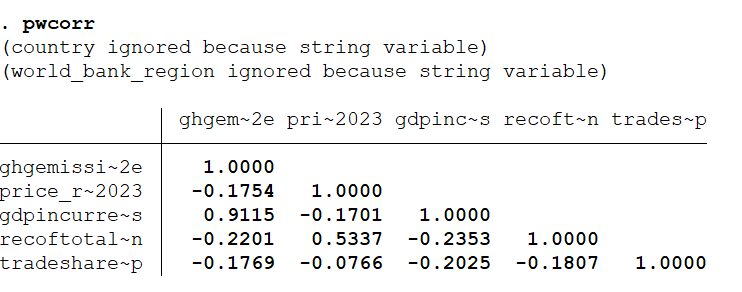
\includegraphics[width=12cm,height=6cm]{ANOVA/1.png} 
    \caption{Pairwise correlation test}
\end{figure}

The Variance Inflating Factor (VIF) checks for the degree of multicollinearity among our variables. Since our VIF is close to 1, it proves that our dataset has almost no multicollinearity.
\begin{figure}[H]
    \centering
    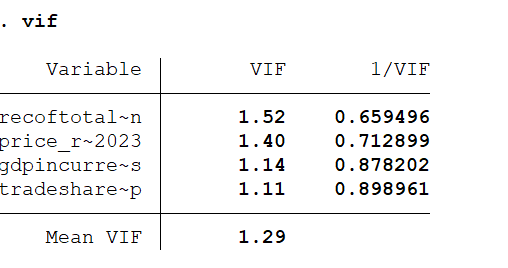
\includegraphics[width=8cm,height=4cm]{ANOVA/2.png} 
    \caption{Variance Inflating Factor (VIF)}
\end{figure}


\section{Model Specification}
\paragraph{}
To assess the impact of Carbon Pricing Mechanisms, and related variables on GHG emissions, we have developed an econometric model. The dependent variable is indicated as GHG emissions (in metric tonnes). The independent variables capture Carbon Pricing Rates under ETS and Carbon Tax schemes, GDP (in current US\$), renewable energy consumption (as a \% of total energy consumption and international trade openness ( as a \% of total GDP).
\begin{center}The following equation is a functional representation of the relationship:\end{center}
\begin{equation}
    C_{i} = f( P_{i}, Y_{i}, RE_{i}, T_{i} )
\end{equation}
Where, i represents the ith country. Ci represents GHG emissions, Pi represents Carbon Pricing Rates(including Carbon Tax and EU ETS scheme), Yi represents Total GDP, REi represents the share of renewable energy consumption, and Ti represents the share of trade activities.
\begin{center}Following is an Econometric model derived from Equation 1\end{center}
\begin{equation}
    C_{i} = \alpha_{o} + \beta_{1}P_{i} + \beta_{2}Y_{i} + \beta_{3}RE_{i} + \beta_{4}T_{i} + u_{i}
\end{equation}

According to the existing literature, the ideal model would show a negative \(\beta_{1}\) such that Carbon Pricing Mechanisms would have a negative impact on emissions, shifting production and consumption of carbon-intensive goods and services to low-carbon alternatives (Roser, 2021). \(\beta_{2}\) should show a positive relationship, indicating that as the GDP of a country increases, it would also increase the demand for energy, hence increasing carbon emissions. \(\beta_{3}\) should indicate a negative relationship between renewable energy consumption and greenhouse gas emissions, indicating a cleaner alternative. \(\beta_{4}\) should show a positive relationship indicating the increase in carbon emissions due to an increase in the production and transport of exported and imported goods.



\section{Methodology}
\paragraph{}
The purpose of this project is to do a multiple linear regression analysis and hypothesis testing to check the statistical significance of the variables, along with the sign of their coefficients.
\newpage
\begin{center}Null and Alternative Hypothesis is as follows:\end{center}
\begin{equation*}
    \text{$H_{o}$}: \beta_{1}=\beta_{2}=\beta_{3}=\beta_{4}=0
\end{equation*}
where there is no relationship between carbon pricing, emissions, and other control variables
\begin{center}
    \text{$H_{A}$}: At least one of the independent variables is not equal to 0 
\end{center}
where there is a relationship between carbon pricing, emissions, and other control variables
\\With the available data, we generate an ANOVA table and observe the t and f statistics and corresponding p values to check the statistical significance of the variables. We also check the sign of coefficients to see if the causal relationship matches that of the existing literature. 
\\From our analysis, we then derive our inferences. 


\section{Analysis}


Following is the ANOVA table from the regression model in Equation 2.
\begin{figure}[H]
    \centering
    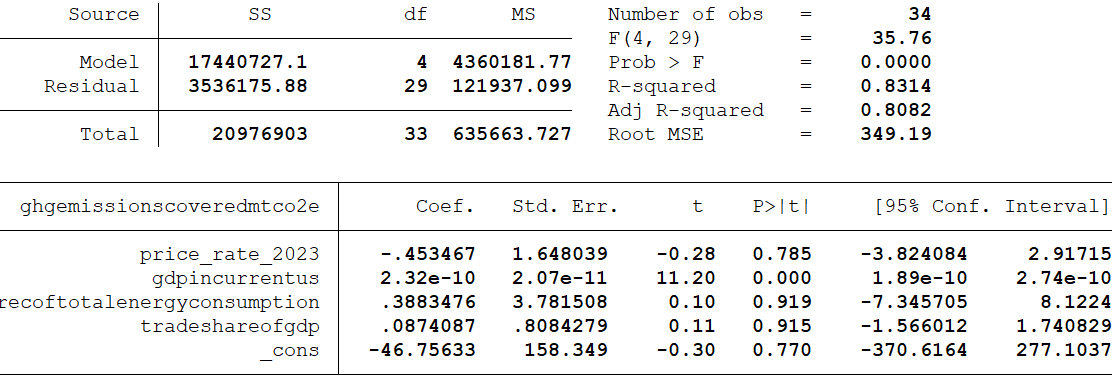
\includegraphics[width=16cm,height=6cm]{ANOVA/3.png} 
    \caption{ANOVA table}
\end{figure}


\textbf{Note:}
\begin{itemize}
    \item Calculated t-value at 1,5,10\% level of significance and 33 degrees of freedom is 2.733, 2.035, 1.692 respectively
    \item Calculated f-value at 1,5,10 \% level of significance and (4,29) degrees of freedom is 4.045, 2.701 and 2.149 respectively

\end{itemize}


\subsection{Individual Significance}
\label{sec:Individual-significance}
The current price rate of Carbon Taxes and ETS schemes has a negative coefficient \(\sim(-0.45)\), indicating an inverse relationship with carbon emissions. The corresponding p-value is 0.785, whereas the calculated t-value is -1.57, which is less than the tabulated t-value. Hence making the variable insignificant.
\\[\baselineskip]
GDP at current US\$ is positively related to carbon emissions \(\sim(2.32x10^{-10})\). The corresponding p-value is at  0, and the calculated t-value is 11.20, greater than the tabulated t-value. Hence making it highly significant.
\\[\baselineskip]
Renewable energy consumption (as a \% of total energy consumption) is positively related to carbon emissions \(\sim(0.38)\). The corresponding p-value is 0.919, whereas the calculated t-value is 0.10, which is less than the tabulated t-value. Hence making the variable insignificant.
\\[\baselineskip]
Trade (as a \% share of total GDP) is also positively related to carbon emissions \(\sim(0.087)\) The corresponding p value is at  0.911, and the calculated t-value is 0.11, less than the tabulated t-value. Hence making the variable insignificant.


\subsection{Overall Significance}
\label{sec:overall-significance}
From the ANOVA table, the overall significance is calculated as 35.76 This is important to consider as it is greater than the calculated f-value at 1,5 and 10\% level of significance. 

\subsection{\(R^{2}\) interpretation}
A high \(R_{2}\) value \(\sim(0.83)\) indicates that the independent variables in our model have been able to explain the variations in our dependent variable to a great extent.

\section{Inference}
From \ref{sec:Individual-significance} and \ref{sec:overall-significance}, we see that the variables in our model is individually insignificant, while it is overall significant. This indicates the collective effect of all the variables on carbon emissions.



\subsection{Carbon Pricing}
The negative impact of carbon prices on Co2 emissions matches with our ideal model, which captures the point that higher carbon prices lead to an increase in energy prices across different sectors and resources, hence causing a fall in carbon emissions (Känzig and Konradt, 2023)


\subsection{Total GDP}
\paragraph{}
The positive impact of a country’s GDP on carbon emissions indicates that as economic activity for a country increases, it leads to increased emissions of carbon during the process. This validates the assumptions of our ideal model. However, the coefficient variable in our analysis is significantly small \(\sim{(2.32x10^{-10})}\). This is because the cross-sectional data of this paper is a study across different countries irrespective of whether they are developed, developing, or least developed economies. Hence canceling out the total effect. There are many dynamics associated which indicate the global inequalities in CO2 emissions. The amount of emissions from high-income countries increases slightly from developed countries, while they decline gradually among developing and less developed countries (Ritchie, 2023).


\subsection{Energy Consumption (Renewables and Fossil Fuels)}
\paragraph{}
From our analysis, the share of renewable energy (RE) consumption has a positive impact on carbon emissions. This is contrary to the assumptions of our ideal model. However, this validates the recent studies which state that renewable energy has a positive impact on CO2 emissions and has still not reached a significant level to reduce the emissions. This directs us to the possibility that Fossil Fuels, along with other sources, still make up the majority of final energy consumption. Moreover, the sustainability of RE varies across different parts of the world, hence making its overall impact uncertain (Zeng et al., 2017). Additionally, energy extraction for RE development is another source of high carbon emissions, hence becoming counterproductive to its very purpose. (Feng, 2022).



\subsection{Trade}
\paragraph{}
While our analysis shows that international trade has a positive impact on CO2 emissions, it is also highly insignificant at the individual level. This is primarily because of two reasons
\begin{enumerate}
    \item The sample size of the countries is small in this context (n=34)
    \item We take into account a mixture of countries from different levels of economic growth, hence affecting the overall impact of trade openness.
\end{enumerate}


\section{Conclusion}

\paragraph{}
In this paper, we aimed to develop a multiple linear regression model to assess the impact of carbon pricing mechanisms on carbon emissions. Additionally, we also included other factors such as economic growth, energy consumption, and trade openness as control variables to provide a comprehensive overview of the complex interplay between policy actions and carbon emissions. Using a sample of 34 countries representing different regions of the world, we found that all our explanatory variables, except for Total GDP, were statistically insignificant. 
\\[.5\baselineskip]
However, our model was overall significant, indicating the interdependence of multiple factors affecting the trajectory of greenhouse gas emissions. Hence, it aimed to contribute to the ongoing discussions on the effectiveness of carbon mechanisms in reducing global carbon emissions. This highlights the need for nuanced approaches, considering this intricate relationship.


\newpage


\begin{flushleft}
    \begin{Large}
     \textbf{Data Sources}
\end{Large}
\end{flushleft}

\begin{enumerate}
    \item \href{https://carbonpricingdashboard.worldbank.org/map_data}{Country, World Bank Region, GHG emissions, and Carbon Price Rates( as of 2023)}

    \item \href{https://data.worldbank.org/}{Total GDP, Share of Renewable Energy Consumption,  and Share of Trade}

    \item \href{https://cepr.org/voxeu/columns/economic-effects-carbon-pricing}{Känzig, D., \& Konradt, M. (2023, August 12). The economic effects of carbon pricing. CEPR.}
\end{enumerate}

\addcontentsline{toc}{section}{References}
\begin{thebibliography}{9}
\printbibliography[title=References]

\bibitem{}
\href{https://ourworldindata.org/carbon-price}{Max Roser (2021) - “The argument for a carbon price”}

\bibitem{}
\href{https://ourworldindata.org/inequality-co2}{Hannah Ritchie (2023) - “Global inequalities in CO2 emissions"}

\bibitem{}
\href{https://cepr.org/voxeu/columns/economic-effects-carbon-pricing}{Känzig, D., \& Konradt, M. (2023, August 12). The economic effects of carbon    pricing. CEPR}

\bibitem{}
\href{https://www.imf.org/en/Publications/fandd/issues/2021/09/five-things-to-know-about-carbon-pricing-parry}{Five Things to Know about Carbon Pricing. (2021, September 2). IMF.}

\bibitem{}
\href{}{Skaredotter, E., \& Ribberheim, O. (2019). A Multivariable Regression Analysis of the Price of Emission Allowances in the EU, KTH Sweden}

\end{thebibliography}



\end{document}